%---------------------------------------------------------------------
%
%                          Editor
%
%---------------------------------------------------------------------

\chapter{Editor}

\section{Funcionamiento y arquitectura}

El editor est� desarrollado en C++ a pesar de no tener el motor integrado debido a la elecci�n de utilizar ImGui, una biblioteca de interfaz de usuario (UI) dise�ada espec�ficamente para C++. Esta elecci�n nos brind� acceso a una amplia gama de funcionalidades esenciales para la creaci�n del editor.

\medskip

En cuanto a su funcionamiento, el editor se compone de tres secciones principales:

\begin{enumerate}
    \item \textit{Gestor de proyectos}: Esta secci�n es la primera en iniciarse y se encarga de crear una configuraci�n espec�fica y un directorio dedicado para cada videojuego que se desee crear.
    
    \item \textit{Ventana de edici�n de scripts}: Desde esta ventana se maneja la creaci�n y edici�n de scripts. Permite a los desarrolladores definir el comportamiento y la l�gica del juego de manera flexible.
    
    \item \textit{Editor principal}: El n�cleo del editor es esta secci�n, donde se lleva a cabo la mayor�a de la creaci�n y edici�n de contenido. Aqu� se manejan las entidades, la jerarqu�a, los componentes y los assets del juego.
\end{enumerate}

El flujo de trabajo del editor comienza con la ventana del gestor de proyectos. Despu�s se traslada a una pila de estados, que determina qu� ventana se debe mostrar y manejar en un momento dado, ya sea la ventana de edici�n de scripts o el editor principal.
Todas las operaciones en el editor se gestionan a trav�s de un bucle principal que se encarga de manejar la entrada del usuario, actualizar el estado de las ventanas y renderizarlas.

\medskip

En el dibujo \ref{fig:funcionamientoEditor} podemos ver dicho flujo.

\medskip

En cuanto al funcionamiento de las ventanas, cada ventana del editor hereda de una clase padre que proporciona el funcionamiento b�sico necesario en ImGui y que sirve como base para definir el comportamiento espec�fico de cada ventana de la escena.

\medskip

En el dibujo \ref{fig:arquitecturaVentanas} observamos esta arquitectura.

\medskip

En cuanto a la gesti�n de entidades, cada una de ellas se identifica mediante un ID �nico. Este ID desempe�a un papel crucial al permitir la distinci�n entre las distintas entidades y se utiliza, por ejemplo, para referenciarlas en scripts. Adem�s, cada entidad puede contener una referencia a su entidad padre o a sus entidades hijas, en caso de que existan relaciones jer�rquicas.

\medskip

Un aspecto importante del sistema de IDs es que tambi�n se utiliza para diferenciar las entidades normales de los prefabs\footnotemark. 

\medskip

Los prefabs se distinguen por tener un ID negativo, lo que les permite ser identificados de manera �nica. Para identificar una entidad como una instancia de un prefab, se modifica el atributo ``PrefabId'' de la entidad, asign�ndole el ID negativo correspondiente al prefab al que est� relacionada.

\begin{figure}[h]
    \centering
    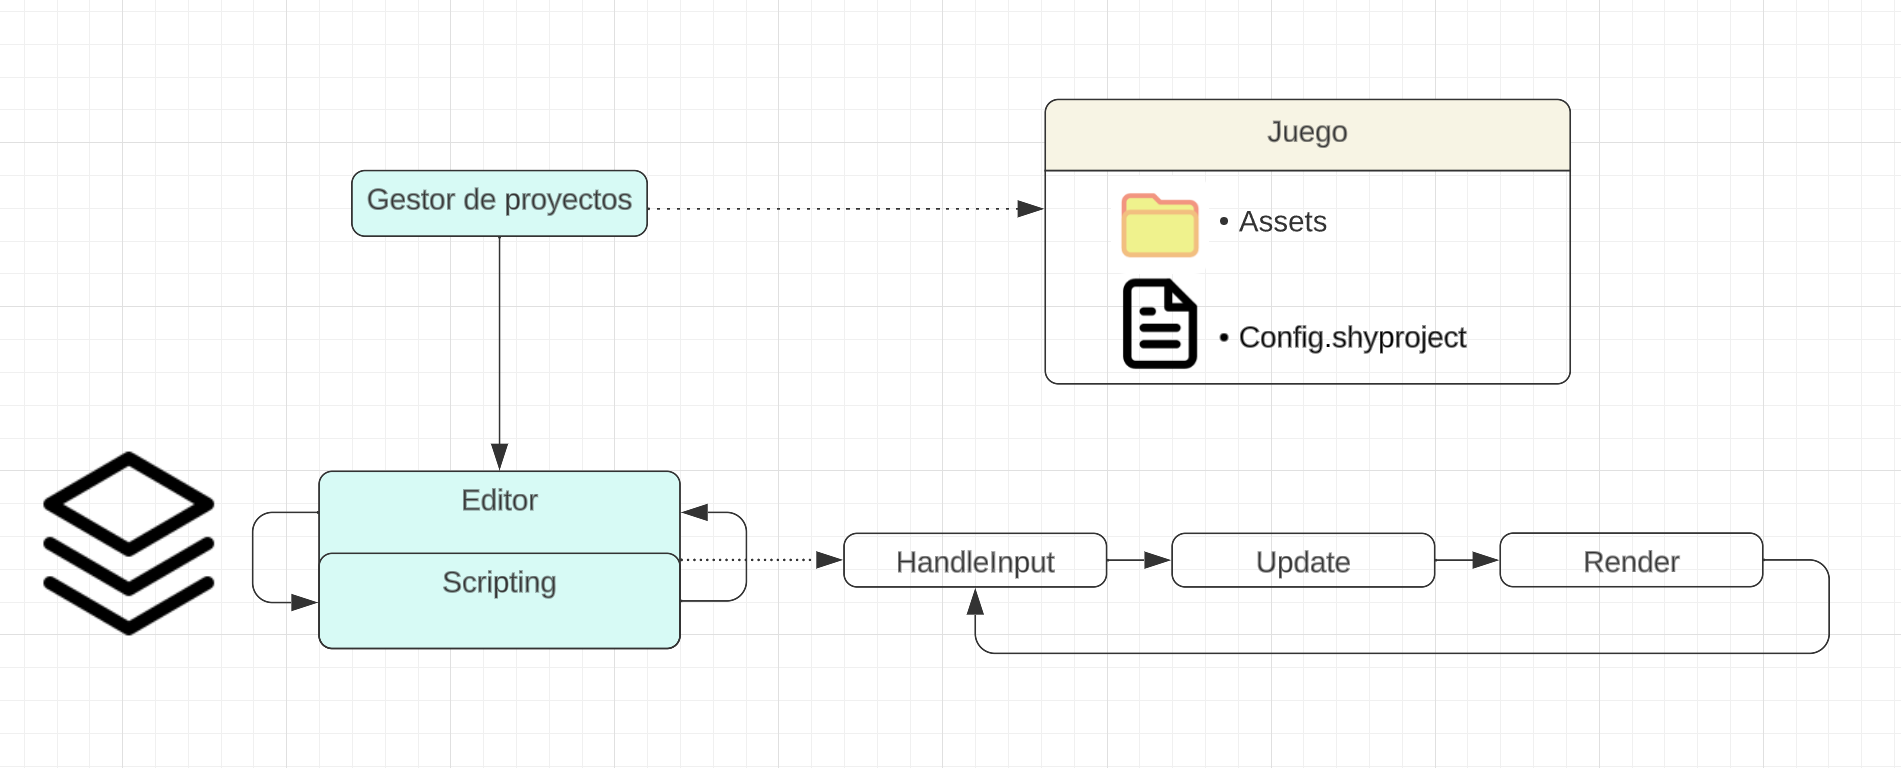
\includegraphics[width=0.6\textwidth]{Imagenes/Vectorial/FuncionamientoEditor.png}
    \caption{Flujo de funcionamiento del editor.}
    \label{fig:funcionamientoEditor}
\end{figure}


\begin{figure}[h]
    \centering
    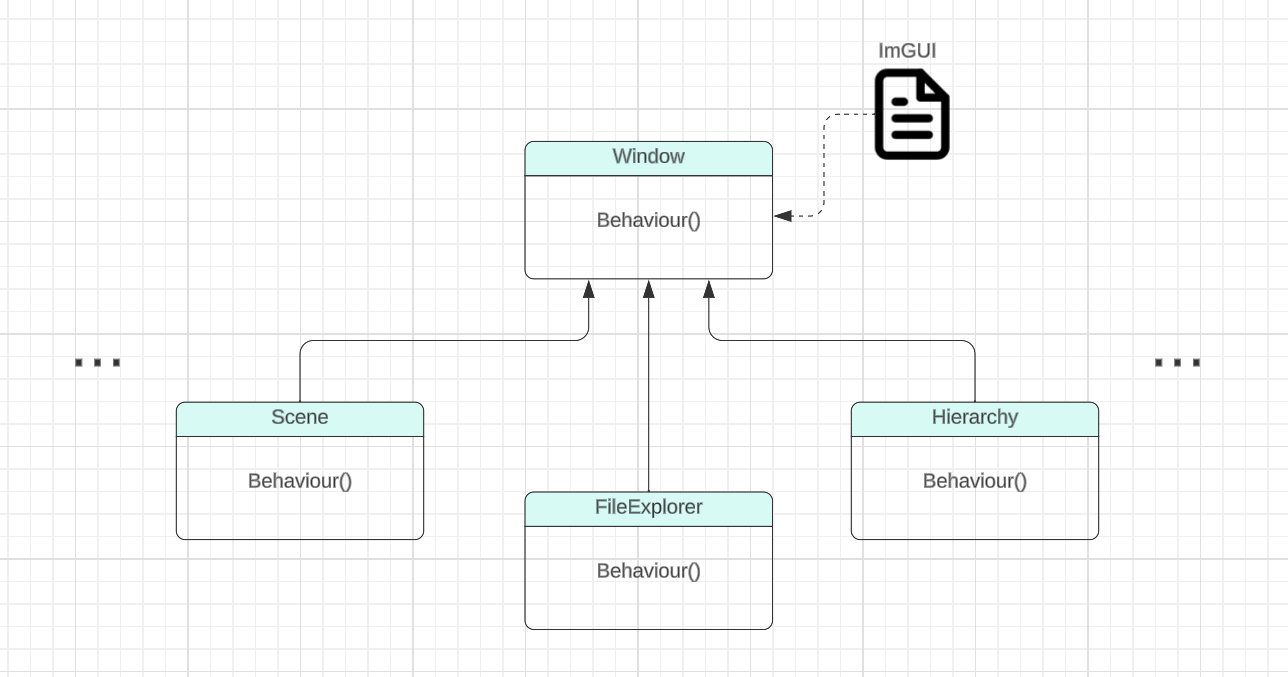
\includegraphics[width=0.6\textwidth]{Imagenes/Vectorial/ArquitecturaVentanas.png}
    \caption{Arquitectura de las ventanas.}
    \label{fig:arquitecturaVentanas}
\end{figure}

\section{Ventana de scripting en el editor}

TODO


\section{Como se leen los componentes a partir de los datos del motor}

Como se mencion� anteriormente en (a�adir referencia al apartado del motor que hable sobre esto), el motor del juego genera archivos en formato JSON que contienen los datos serializados de los componentes, sus atributos y su tipo correspondiente.

\medskip

Los datos en formato JSON se interpretan y se utilizan para construir objetos de tipo ``Component'' en el editor. Cada objeto ``Component'' contiene un vector de objetos llamados ``Attribute'', y estos a su vez almacenan un valor que se ajusta al tipo de atributo le�do en el archivo JSON (int, float, Vector2...). Las entidades contienen un vector con los componentes que se le hayan a�adido y sus valores se pueden modificar desde la ventana Components del editor.

\medskip

En la imagen \ref{fig:datosEditor} se puede observar el funcionamiento de la lectura.

\begin{figure}[h]
    \centering
    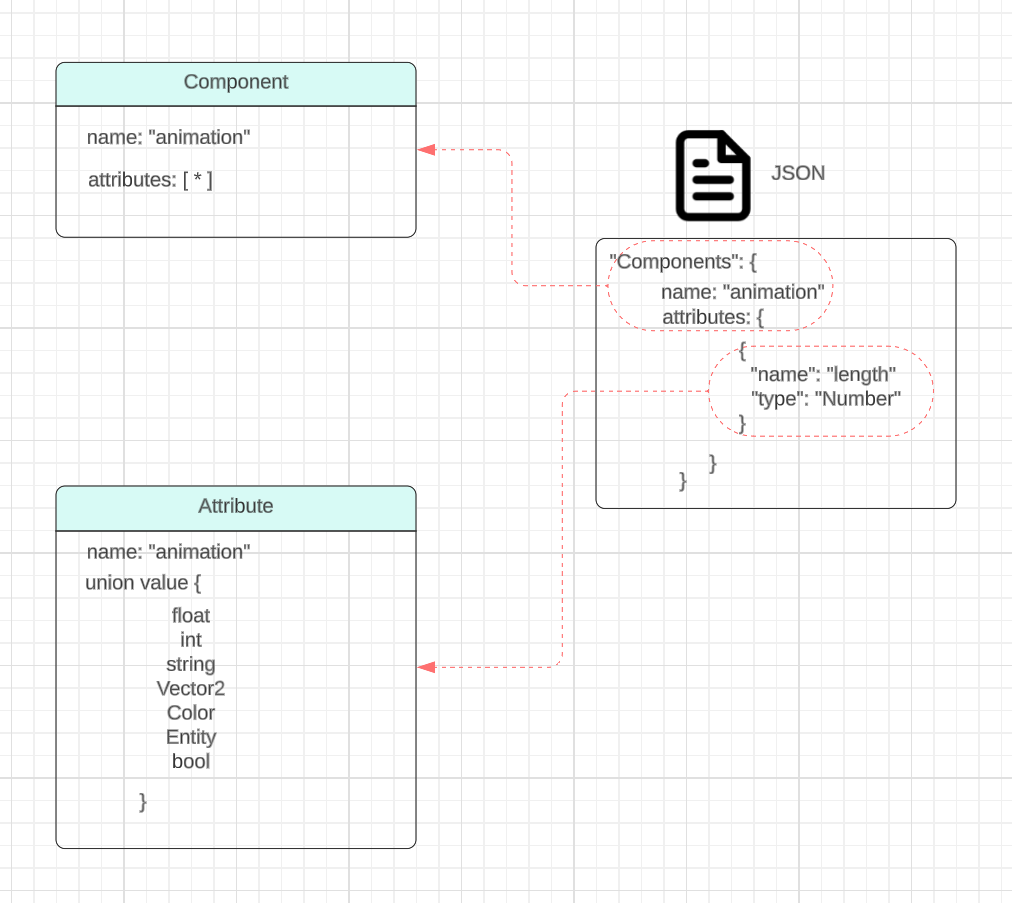
\includegraphics[width=0.6\textwidth]{Imagenes/Vectorial/LecturaComponentesEditor.png}
    \caption{Lectura de componentes del motor en el editor.}
    \label{fig:datosEditor}
\end{figure}


\footnotetext{Un prefab es una entidad predefinida que se puede instanciar en la escena. Contiene una configuraci�n espec�fica y puede reutilizarse en diferentes partes del juego para simplificar el proceso de dise�o y desarrollo. Adem�s, modificar un prefab modifica tambi�n todas sus instancias en la escena.} 

%------------------------------------------------  --------------------------------------------


